\documentclass{article}
% main document, called main.tex
\usepackage{tikz}
\usetikzlibrary{external}
\usetikzlibrary{math}
\tikzexternalize % activate!
\begin{document}
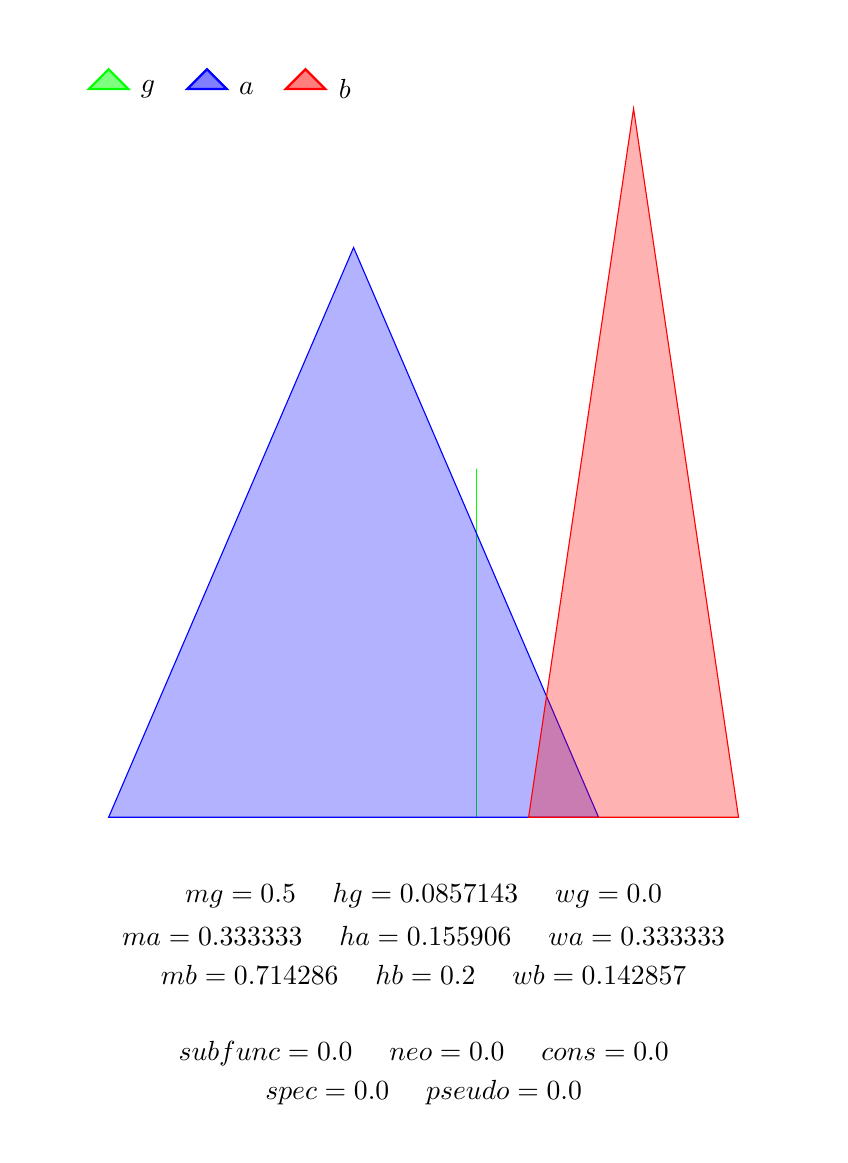
\begin{tikzpicture}
%\draw[blue, very thick] (0,0) rectangle (3,2);

\tikzmath{
\mg = 0.5;
\hg = 0.0857143;
\wg = 0.0;
\ma = 0.333333;
\ha = 0.155906;
\wa = 0.333333;
\mb = 0.714286;
\hb = 0.2;
\wb = 0.142857;
\mgadjusted = 5.6666658888890185;
\hgadjusted = 4.428571999999999;
\wgadjusted = 0.0;
\maadjusted = 4.111107481482087;
\haadjusted = 7.23624;
\waadjusted = 3.1111074814820863;
\mbadjusted = 7.666668222221963;
\hbadjusted = 9.0;
\wbadjusted = 1.3333317777780371;
\zeroheight = 0;
\pneo = 0.0;
\psubfunc = 0.0;
\pcons = 0.0;
\pspec = 0.0;
\ppseudo = 0.0;
}



\draw[white, fill=white, ultra thick, fill opacity=1] (0, -4) -- (10, -4) -- (10, 10) -- (0, 10) -- cycle;
\draw[green, fill=green, thin, fill opacity=0.5] (\mgadjusted - \wgadjusted, \zeroheight) -- (\mgadjusted + \wgadjusted, \zeroheight) -- (\mgadjusted,\hgadjusted) -- cycle;
\draw[blue, fill=blue, thin, fill opacity=0.3] (\maadjusted - \waadjusted, \zeroheight) -- (\maadjusted + \waadjusted, \zeroheight) -- (\maadjusted,\haadjusted) -- cycle;
\draw[red, fill=red, thin, fill opacity=0.3] (\mbadjusted - \wbadjusted, \zeroheight) -- (\mbadjusted + \wbadjusted, \zeroheight) -- (\mbadjusted,\hbadjusted) -- cycle;

%legend
\draw[green, fill=green, thick, fill opacity=0.5] (0.75,9.25) -- (1.25,9.25) -- (1,9.5) -- cycle;
\node[] at (1.5,9.25) { $g$};

\draw[blue, fill=blue, thick, fill opacity=0.5] (2,9.25) -- (2.5,9.25) -- (2.25,9.5) -- cycle;
\node[] at (2.75,9.25) { $a$};

\draw[red, fill=red, thick, fill opacity=0.5] (3.25,9.25) -- (3.75,9.25) -- (3.5,9.5) -- cycle;
\node[] at (4,9.25) { $b$};

\node[] at (5,-1) {$mg = \mg$ \quad  $hg = \hg$ \quad  $wg = \wg$};
\node[] at (5,-1.5) {$ma = \ma$ \quad  $ha = \ha$ \quad  $wa = \wa$};
\node[] at (5,-2) {$mb = \mb$ \quad  $hb = \hb$ \quad  $wb = \wb$};


\node[] at (5,-3) {$subfunc = \psubfunc$ \quad  $neo = \pneo$ \quad  $cons = \pcons$};
\node[] at (5,-3.5) { $spec = \pspec$ \quad $pseudo = \ppseudo$};




\end{tikzpicture}

\end{document}